\documentclass[letterpaper, 12pt]{article}

\usepackage{geometry}
 \geometry{
 letterpaper,
 total={170mm,257mm},
 left=20mm,
 top=20mm,
 bottom=20mm
 }
\usepackage{graphicx} % Required for inserting images
\usepackage{authblk}
\usepackage{amssymb}
\usepackage{lipsum}
\usepackage{float}
\usepackage{times}
\usepackage{amsmath}
\usepackage[format=plain,
            labelfont={bf,it},
            textfont=it]{caption}
\captionsetup{justification=raggedright,singlelinecheck=false}
\usepackage{ragged2e}
\usepackage{longtable}
\usepackage{comment}
\usepackage{setspace}
\usepackage{fancyhdr}
\usepackage{titlesec}
\usepackage[hyperindex,breaklinks]{hyperref}
\hypersetup{
    colorlinks=true,
    linkcolor=blue,
    filecolor=magenta,      
    urlcolor=blue,
    pdftitle={Overleaf Example},
    pdfpagemode=FullScreen,
    }
% \usepackage{background} % add COSIG logo to page
\usepackage[T1]{fontenc}
\usepackage{helvet}
\renewcommand{\familydefault}{\sfdefault}
\pagenumbering{gobble}
\usepackage[skip=10pt plus1pt, indent=40pt]{parskip}

\titlespacing*{\section}
{0pt}{1.5ex plus 1ex minus .2ex}{1.3ex plus .2ex}

\renewcommand\Authfont{\fontsize{12}{14.4}\selectfont}
\renewcommand\Affilfont{\fontsize{9}{10.8}\itshape}
 
\begin{document}
\flushleft

\includegraphics[width=0.5\textwidth]{img/home/241017_final_logo_mockup.png}

\section*{Common dismissive responses to integrity concerns}
\addcontentsline{toc}{section}{Common dismissive responses to integrity concerns}
\textit{Last updated: 7 April 2025}

Authors, editors and research integrity officers often respond dismissively to valid publication integrity concerns. This guide covers a handful of such responses commonly encountered by post-publication peer reviewers and provides frameworks for responding to them.

\subsection*{``We do not respond to anonymous complaints.''\newline 
``Please share your name and email address and we will send you the data.''}

Post-publication peer reviewers often become targets for harassment and litigation. Researchers risk jeopardizing their careers by raising integrity issues in the publications of prominent scientists in their field. Anonymity and pseudonymity protect post-publication peer reviewers from retaliation. Many post-publication peer reviewers would likely not share their on observations if they were required to publicly share their identities. For similar reasons, anonymity of peer reviewers has long been \href{https://doi.org/10.1038/6295}{accepted as standard} in pre-publication peer review pipelines. 

In their \href{https://doi.org/10.24318/cope.2019.2.25}{flowchart on responding to integrity concerns raised directly with editors}, the Committee on Publication Ethics (COPE) advises ``[sometimes] the whistleblower may prefer
to remain anonymous. It is important not to try to `out' people who wish to be anonymous.'' COPE also \href{https://doi.org/10.24318/Z9gtPzCa}{recommends} that anonymous whistleblowers ``should be treated courteously and the complaint investigated appropriately, as it would be if the complaint were from another source''.

Moreover, a peer reviewer's anonymity does not prevent authors from sharing original images or data. Instead of sending data to a single commenter over email, authors can upload data to a data sharing service like \href{https://datadryad.org/stash}{Dryad}, \href{https://figshare.com/}{figshare}, \href{https://zenodo.org/}{Zenodo} or \href{https://osf.io/}{Open Science Framework} and share a link to the dataset publicly, allowing others beyond the original commenter to access their data.

\subsection*{``You are not a scientist and are thus not qualified to review this work.''\newline``Please provide an article that you have published on this subject.''}

Publication integrity concerns should be evaluated based on the substance of the concern, not the credentials or experience of the commenter raising the concern.

\subsection*{``The images shown in this article are representative/illustrative in nature and are not actual data.''}

\href{https://doi.org/10.1007/978-1-62703-056-4_1}{Images are data}. Whether or not the images in an article are presented as representative of a larger set of experimental observations, images are present to convey information to the reader. The presence of problematic images implies that the information they convey is inaccurate and can shake readers' confidence in the veracity of other information presented in the article. 

Moreover, images provide valuable information for those looking to reproduce experiments, setting expectations for what samples should look like if the experiments are performed correctly. If these images are not faithful representations of an experimental condition, it limits the reproducibility of a published work.

\subsection*{``These images were published a long time ago, when digital image manipulation was not possible.''\newline``These images were collected on analog technology and thus could not have been manipulated.''}

Digital manipulation of images has been regarded as a means for distortion of data presented in scientific articles since \href{https://doi.org/10.1002/(SICI)1096-9896(199711)183:3%3C253::AID-PATH927%3E3.0.CO;2-P}{as early as 1997} (see additional commentary on the topic \href{https://doi.org/10.1083/jcb.200406019}{published in 2004}).

Outside of the scientific literature, manipulation of photographs is \href{https://iisjoa.org/sites/default/files/iisjoa/2017/PDF/11.%20Jitendra%20Sharma%20&%20Rohita%20Sharma.pdf}{as old as photography itself} (consider the practice of \href{https://en.wikipedia.org/wiki/Spirit_photography}{spirit photography} or \href{https://en.wikipedia.org/wiki/Exaggeration_postcard}{tall-tale postcards}). Retractions have even been issued for apparent image manipulation in scientific articles published well before digital image manipulation software became widely available. For instance, \href{https://doi.org/10.1128/jvi.56.1.284-292.1985}{Fusco et al. (1985)} was \href{https://doi.org/10.1128/jvi.02169-17}{retracted in 2018} for apparent manipulation of images of \href{https://doi.org/10.1093/nar/7.6.1541}{RNA dot blots}.

\begin{figure}[h!tbp]
    \centering
    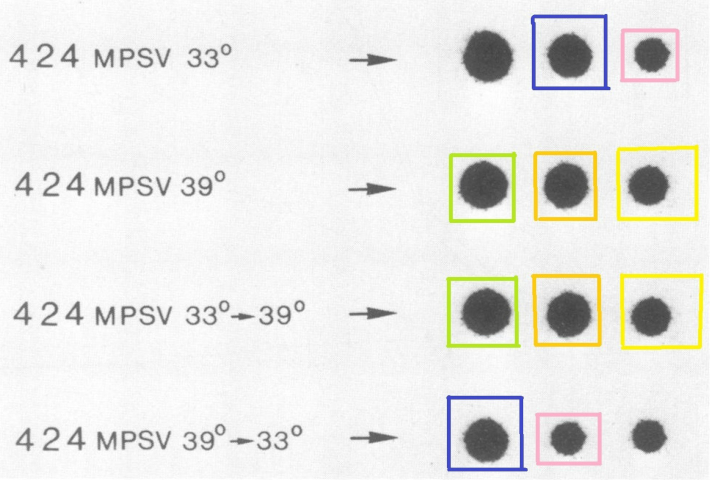
\includegraphics[width=0.8\textwidth]{img/responses/imgur-ESa5N4V_scaled.jpg}
    \caption*{\href{https://doi.org/10.1128/jvi.56.1.284-292.1985}{Fusco et al. (1985)} reports on RNA quantification experiments with dot blot images that have apparently been manipulated. Colored boxes indicate portions of the image that are identical to one another. Adapted from Figure 8 of Fusco et al. by \href{https://pubpeer.com/publications/67130CFDA6D3D4F59D463598ACE835\#3}{an anonymous PubPeer commenter}.}
\end{figure}

\pagebreak

\subsection*{``This comment concerns one image among dozens with no issues in this article.''}

When one image or piece of data in one part of an article has concerning irregularities, it is reasonable for readers to have doubts about other data reported in the article.

Consider a hypothetical instance where there are extensive internal duplications in a published image suggestive of deliberate manipulation. Readers cannot know who among the authors was responsible for this manipulation, their motivations, nor what other data in the article may have been manipulated. When any signs of manipulation are present, readers are left wondering whether there is more instances of manipulation that are impossible to discover by examining the published article alone.

\subsection*{``We did not use tortured phrases, just alternative scientific terminology.''}

There are instances where using scientific nomenclature that departs from more commonly-used language is acceptable. Using \href{https://pubpeer.com/search?q=%22bosom+disease%22}{``bosom disease''} in place of ``breast cancer'' is not one of these instances.

See the section on tortured phrases in the \href{https://osf.io/ntcb4}{COSIG guide on textual plagiarism}.

\subsection*{``There are no duplicated regions in the image in question; these regions only appear similar because of structural similarities in the sample.''}

There is expected to be some similarity in appearance between particles in a sample, cells in culture, physiological structures in a tissue sample, bands in a Western blot, etc. However, large regions of an image actually depicting different objects are unlikely to be identical down to the pixel. If authors believe that similarities between images or regions of an image are in fact due to chance alone, they can alleviate concerns by providing the original, high-resolution images corresponding to those shown in the article.

\begin{figure}[h!tbp]
    \centering
    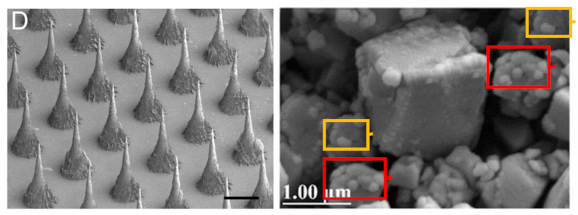
\includegraphics[width=\textwidth]{img/responses/yu_vs_mohaghegh_0.PNG}
    \caption*{\href{https://doi.org/10.1073/pnas.1505405112}{Yu et al. (2015)} show a scanning electron microscope (SEM) image (left, adapted from Figure 4D) of a microneedle array cast from a precisely-fabricated silicon mold. Each microneedle is designed to have the same shape as the next. However, no two microneedles appear exactly alike. On the other hand, \href{https://doi.org/10.1007/s10853-015-9003-3}{Mohaghegh et al. (2015)} report synthesizing crystal nanoparticles by precipitation from solution, for which it would be impossible to exactly control the shape of the synthesized product. However, one of the images of these nanoparticles shown in the article (right, adapted from Figure 3A by \href{https://pubpeer.com/publications/7BE7C2A93C385F700F1C6B5BC90294\#1}{Reese Richardson}) contains large regions that are identical to one another (highlighted by colored boxes). It is highly unlikely that any two nanoparticles in this sample actually appeared this similar to one another.}
\end{figure}

\end{document}